\documentclass{article}
\usepackage{amsmath}
\usepackage{tikz}
\usetikzlibrary{positioning}
\title{Ciclo Impar o Bipartito}
\author{Daniel Bustos}
\date{11 de mayo 2024}

\begin{document}

\section*{Daniel Bustos, Ciclo Impar o Bipartito}

\textbf{1a)} Queremos demostrar que: \textbf{$vw$ es un puente de $G \leftrightarrow$ $vw$ no pertenece a ningún ciclo de $G$}. Probemos la ida y la vuelta:
\begin{itemize}


\item \textbf{ $vw$ es un puente de $G \rightarrow vw$ no pertenece a ningún ciclo de $G$}

Si $vw$ es un puente, quiere decir que removerla aumenta la cantidad de partes conexas. Observemos que si $vw$ perteneciese a un ciclo, entonces al sacarla, no estaríamos generando ninguna parte conexa nueva. Por virtud de ser ciclo, luego de remover a $vw$ ahora nos quedaría un camino simple, que sigue siendo claramente conexo. Luego, se sigue que $vw$ no pertenece a ningún ciclo de $G$.

\item \textbf{$vw$ no pertenece a ningún ciclo de $G \rightarrow vw$ es un puente de $G$}

Si $vw$ no pertenece a ningún ciclo, quiere decir que la arista es solo parte de un camino. Al remover la arista, necesariamente nos quedarán dos partes del camino, entre sí desconexas, luego $vw$ es un puente.
\end{itemize}
\begin{figure}[h]
    \centering
    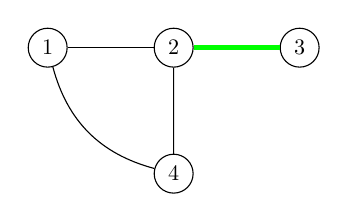
\begin{tikzpicture}[scale=0.8,transform shape]
        \node[circle,draw] (1) at (0,0) {1};
        \node[circle,draw] (2) at (2,0) {2};
        \node[circle,draw] (3) at (4,0) {3};
        \node[circle,draw] (4) at (2,-2) {4};
        
        \draw (1) -- (2);
        \draw[green,line width = 2pt] (2) -- (3);
        \draw (2) -- (4);
        
        \draw (1) to [bend right] (4);
    \end{tikzpicture}
    \hspace{1cm}
    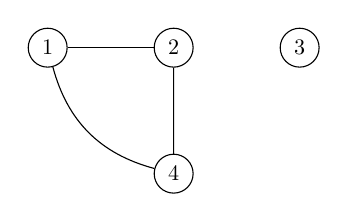
\begin{tikzpicture}[scale=0.8,transform shape]
        \node[circle,draw] (1) at (0,0) {1};
        \node[circle,draw] (2) at (2,0) {2};
        \node[circle,draw] (3) at (4,0) {3};
        \node[circle,draw] (4) at (2,-2) {4};
        
        \draw (1) -- (2);
        \draw (2) -- (4);
        \draw (1) to [bend right] (4);
    \end{tikzpicture}
    \caption{Grafo con y sin arista puente, se observa que el puente no podria pertenecer al ciclo}
\end{figure}
\textbf{b)} Queremos demostrar que: \textbf{$vw \in E(G) \setminus E(T) \rightarrow v$ es un ancestro de $w$ en $T$ o viceversa.}

Dado que $T$ es un árbol DFS, todos los vértices que estén en $G$ pero no en $T$ son backedges por definición. Luego, al haber una backedge $vw$, se sigue que $v$ es ancestro de $w$ o $w$ de $v$ en $T$.\\


\begin{center}

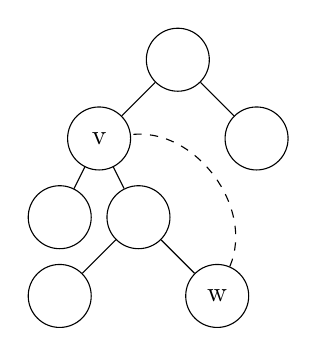
\begin{tikzpicture}[every node/.style={circle, draw, minimum size=0.8cm}]
    \node (A) at (0,0) {};
    \node (B) at (-1,-1) {v};
    \node (C) at (1,-1) {};
    \node (D) at (-1.5,-2) {};
    \node (E) at (-0.5,-2) {};
    \node (F) at (0.5,-3) {w};
    \node (G) at (-1.5,-3) {};
    
    \foreach \from/\to in {A/B, A/C, B/D, B/E, E/F, E/G}
        \draw (\from) -- (\to);
    
    % Backedge
    \draw[dashed] (F) to[bend right=60] (B);
\end{tikzpicture}
\end{center}

Para una respuesta un poco mas satisfactoria: El arbol DFS registra todas las aristas por las que paso el algoritmo , siempre y cuando el nodo al que este avanzando no haya sido procesado ya por el algoritmo. Si existen aristas que no estan en el arbol DFS, quiere decir que el algoritmo \textit{ volvio a un nodo por el que ya habia pasado antes}, por lo tanto no guardo esa arista. Si pudo volver por un nodo que ya habia pasados antes, quiere decir que recorrio un ciclo, y dado que el algoritmo es secuencial, el nodo repetido debe ser antecesor a todos los nodos por los que paso despues de el . De ahi se sigue que esta backedge conecta a un elemento v con algun ancestro w (o viceversa) \\


\textbf{c)}
Sea $vw \in E(G)$ una arista tal que el nivel de $v$ en $T$ es menor o igual al nivel de $w$ en $T$.
Demostrar que: \textbf{$vw$ es puente $\leftrightarrow v$ es el padre de $w$ en $T$ y ninguna arista de $G \setminus \{vw\}$ une a un descendiente de $w$ (o a $w$) con un ancestro de $v$ (o con $v$)}.\\

Probemos la ida y la vuelta :\\

\begin{itemize}

\item \textbf{$vw$ es puente $\rightarrow  v$ es el padre de $w$ en $T$ y ninguna arista de $G \setminus \{vw\}$ une a un descendiente de $w$ (o a $w$) con un ancestro de $v$ (o con $v$)}

Sabemos por el item (a) que $vw$ no esta en ningun ciclo, lo cual satisface la 2da condicion, ya que si hubiese aristas que uniesen desdendientes de $w$ ( o a $w$) con un ancestro de $v$ (o con $v$) distintas a $vw$, podriamos formar un ciclo. \\
Dado que $vw$ es puente, sabemos que remover esta arista necesariamente debe generarnos mas partes conexas. Pensemos en los distintos casos de las posibles diferencias de alturas entre ambos:

\item si altura(v) = altura(w) entonces sacar la arista no nos generia mas partes conexas, ya que siempre podemos recorrer el arbol hacia arriba para llegar de v a w. Luego sus alturas no pueden  coincidir:
\begin{figure}[h]
\begin{center}
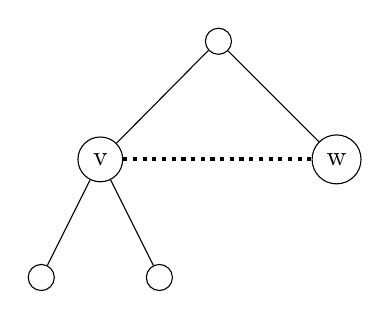
\begin{tikzpicture}[level distance=1.5cm,
                    level 1/.style={sibling distance=3cm},
                    level 2/.style={sibling distance=1.5cm}]
  \node[circle,draw] (root) {}
    child {node[circle,draw] (a) {v} 
      child {node[circle,draw] (b) {}}
      child {node[circle,draw] (c) {}}}
    child {node[circle,draw] (d) {w}};

  % Cross edge
  \draw[dotted,line width = 1.5pt] (a) -- (d);
\end{tikzpicture}
\caption{Se observa que al remover el vertice que los conecta, la cantidad de partes conexas en el grafo asociado  no cambia}
\end{center}
\end{figure}

\item  Como $\text{altura}(v) < \text{altura}(w)$ y sabemos que no se forman ciclos, entonces necesariamente $v$ debe ser el padre de $w$, ya que de otra forma se nos formaría un ciclo, y sabemos que esto no puede ocurrir porque $vw$ es una arista puente, demostramos asi la ida.
\begin{figure}[h]
\centering
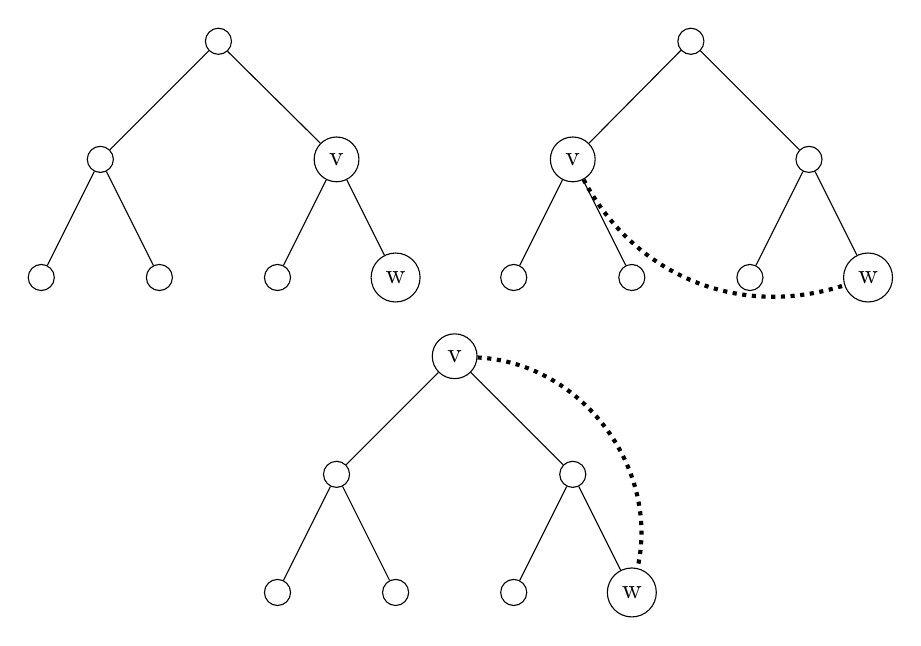
\begin{tikzpicture}[level distance=1.5cm,
                    level 1/.style={sibling distance=3cm},
                    level 2/.style={sibling distance=1.5cm}]
  % First graph
  \begin{scope}[shift={(0,0)}]
    \node[circle,draw] {}
      child {node[circle,draw] {}
        child {node[circle,draw] {}}
        child {node[circle,draw] {}}}
      child {node[circle,draw](v) {v}
        child {node[circle,draw] {}}
        child {node[circle,draw] (w) {w}}};
  \end{scope}

  % Second graph
  \begin{scope}[shift={(6,0)}]
    \node[circle,draw] {}
      child {node[circle,draw] (v2) {v}
        child {node[circle,draw] {}}
        child {node[circle,draw] {}}}
      child {node[circle,draw] {}
        child {node[circle,draw] {}}
        child {node[circle,draw] (w2) {w}}};
   
  \draw[dotted,line width = 1.5pt]  (v2) to[bend right=40] (w2);
  \
  \end{scope}
	\begin{scope}[shift={(3,-4)}]
    \node[circle,draw] (v3){v}
      child {node[circle,draw]  {}
        child {node[circle,draw] {}}
        child {node[circle,draw] {}}}
      child {node[circle,draw] {}
        child {node[circle,draw] {}}
        child {node[circle,draw] (w3) {w}}};
   
  \draw[dotted,line width = 1.5pt]  (v3) to[bend left=50] (w3);
    
  \end{scope}  
  
\end{tikzpicture}
\caption{El unico caso donde no se genera un ciclo, es cuando $v$ es padre de $w$. Notese que un arbol DFS nunca tiene cross edges, lo probamos en (b) . El segundo dibujo es meramente ilustrativo}
\end{figure}

\item \textbf{$ v$ es el padre de $w$ en $T$ y ninguna arista de $G \setminus \{vw\}$ une a un descendiente de $w$ (o a $w$) con un ancestro de $v$ (o con $v$) $\rightarrow vw$ es puente }
 Es facil ver que en este caso vw es arista puente, ya que no hay ninguna otra manera de acceder a w o los nodos que estan por debajo suyo, desde v o algun ancestro suyo, a menos que sea a traves de $vw$ . Luego si removiesemos esta arista, tendriamos mas partes conexas que con las que empezamos. Por lo tanto $vw$ es una arista puente.
\end{itemize}


\end{document}
